% Drawing 81/03-8 -- folder 81, batch 03, archive page 53 (PDF page 54).
% Transcription: au milieu de la feuille, un croquis au crayon repassé à l'encre : deux lobes marqués « mon » et « mon », séparés par une bande à deux traits parallèles, avec en haut de la bande deux flèches épaisses de sens contraires, l'une au-dessus de l'autre.
% Kind: two lobes joined by a band (mon, mon). Method 2 (schematic redraw from the facsimile). Status: partial.
% Notes: Two lobes in pencil, both marked « mon », joined by a band bounded by two pencil strokes; in ink, at the top of the band, two heavy arrows one above the other, the upper pointing right, the lower pointing left. Nothing at the foot of the band. Left out: a small ink tick by the right-hand « mon ». Still differs: the lobes are smooth curves through points read on his outlines; the arrows are schematic. The note of the transcription says « une double flèche au-dessus »: a pair of opposite arrows. Redrawn 2026-11-10 (issue 128): to check again.
% Coordinates: 1 unit = 1 mm = 1/100 of the crop width (bbox in page fractions: [0.42, 0.4, 0.62, 0.47]).
% Redrawn by Claude (claude-fable-5-2), issue #128, 2026-11-10; not checked by a human; not compiled (no TeX in the session).
% Rights: reproduces part of the work -- behind RENDER_TRANSCRIPTS, never published by itself.
\documentclass[tikz,border=3pt]{standalone}
\usepackage{amsmath,amssymb}
\usetikzlibrary{patterns,arrows.meta}
\tikzset{pencil/.style={black!45}, struck/.style={black!35}, mpt/.style={circle,draw,inner sep=1.3pt}, pt/.style={circle,fill,inner sep=0.9pt}, opt/.style={circle,draw,fill=white,inner sep=1.1pt}}
\begin{document}
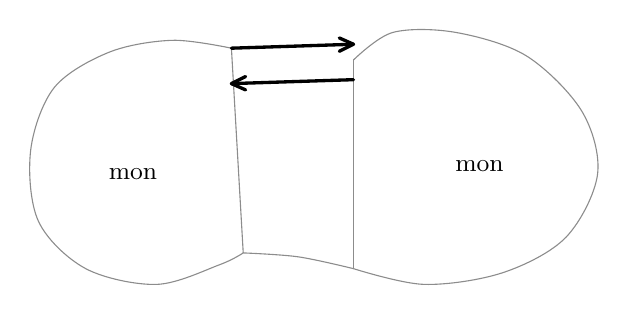
\begin{tikzpicture}[x=1mm,y=1mm,line cap=round,line join=round,font=\scriptsize]
\draw[pencil] plot[smooth, tension=0.55] coordinates {(45.5,-17) (38,-16) (30,-17.5) (23,-22) (20,-30) (21,-39) (27,-45) (36,-47) (44,-44.5) (47,-43)};
\draw[pencil] plot[smooth, tension=0.55] coordinates {(61,-18.5) (66,-15) (74,-15) (83,-18) (90,-25) (92,-33) (88,-41) (80,-45.5) (70,-47) (61,-45)};
\draw[pencil] plot[smooth, tension=0.55] coordinates {(47,-43) (54,-43.5) (61,-45)};
\draw[pencil] (45.5,-17) -- (47,-43);
\draw[pencil] (61,-18.5) -- (61,-45);
\draw[very thick] (45.5,-17) -- (61,-16.5);
\draw[very thick] (59.2,-15.7) -- (61,-16.5) -- (59.2,-17.4);
\draw[very thick] (61,-21) -- (45.5,-21.5);
\draw[very thick] (47.3,-22.3) -- (45.5,-21.5) -- (47.3,-20.6);
\node[inner sep=1pt] at (33,-33) {\small mon};
\node[inner sep=1pt] at (77,-32) {\small mon};
\end{tikzpicture}
\end{document}
